% Flipping a coin
% Author: cis
\documentclass[border=10pt,varwidth]{standalone}
\usepackage{tikz}
\usetikzlibrary{calc, shapes, backgrounds}
\usepackage{amsmath, amssymb}
\pagecolor{white!50!white!50!white}
\begin{document}
\tikzset{
  head/.style = {fill = orange!90!blue,
                 label = center:\textsf{\Large H}},
  tail/.style = {fill = blue!70!yellow, text = black,
                 label = center:\textsf{\Large T}}
}
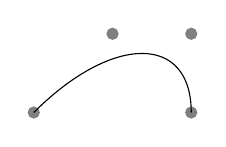
\begin{tikzpicture}
\filldraw [gray] (0,0) circle (2pt)
(1,1) circle (2pt)
(2,1) circle (2pt)
(2,0) circle (2pt);
\draw (0,0) .. controls (1,1) and (2,1) .. (2,0);
\end{tikzpicture}
\end{document}
